% this file is called up by thesis.tex
% content in this file will be fed into the main document

%: ----------------------- introduction file header -----------------------
\chapter{Musiktherapeutische Stimmarbeit}
\label{chapter:musiktherapeutische_stimmarbeit}
\setlength{\epigraphwidth}{8.0cm}
\epigraph{Success depends upon previous preparation, and without such preparation there is sure to be failure.}{Confucius}
\ifpdf
    \graphicspath{{3_experimental_platform/figures/PNG/}{3_musiktherapeutische_stimmarbeit/figures/PDF/}{3_musiktherapeutische_stimmarbeit/figures/}}
\else
    \graphicspath{{3_musiktherapeutische_stimmarbeit/figures/EPS/}{3_musiktherapeutische_stimmarbeit/figures/}}
\fi
% ----------------------------------------------------------------------
%: ----------------------- introduction content -----------------------
% ----------------------------------------------------------------------
\lettrine{I}{n} this chapter, we introduce 



\section{Hardware}
\label{section_experimental_platform_hardware}

\section{Unmanned Aerial Vehicle}
\label{section_experimental_platform_hardware_uav}



\begin{table}[t]
\caption{Platform components and weight}
\label{table_platform_weight}
\begin{center}
\begin{tabular}{l|c}
  \textbf{Component} & \textbf{Weight (g)} \\
  \hline
  2 Hokuyo UTM 30lx & 426 \\
  IMU XSens MTi & 54 \\
  SensorBoard  & 41 \\
  AtomBoard incl. case and WiFi antennas & 126 \\
  GNSS receiver incl. case & 97 \\
  GNSS antenna & 17 \\
\% GNSS antenna cable \& mount & 16 \\
  Shielding (aluminum foil) & 15 \\ \hline
  \textbf{Sum payload} & \textbf{792} \\
  \\

  Payload & 792 \\
  LiPo 4S 16.8V 5Ah & 511 \\
  Mikrokopter Okto2 & 1180 \\ \hline
  \textbf{Sum platform} & \textbf{2483} \\
\end{tabular}
\end{center}
\end{table}

\section{On-Board computing}
\label{section_experimental_platform_hardware_computers}

\section{Inertial Navigation System}
\label{section_experimental_platform_hardware_ins}

...them with 10Hz GNSS PVT\footnote{position, velocity, time} solutions. Because the MEMS-grade IMU exhibits a drift of more tha

\section{LIDAR sensors}
\label{section_experimental_platform_hardware_lidar}



\section{Electromagnetic interference}
\label{section_experimental_platform_hardware_interference}



\section{Software}
\label{section_experimental_platform_software}

\begin{table}
\caption{The TCP/IP-based protocol for communication between rover and base.}
\label{table_protocol}
\begin{center}
\begin{tabular}{l c l}
  \textbf{Message} & \textbf{Direction} & \textbf{Description} \\ \hline
  \parbox[t]{3cm}{UAV status} & Base $\leftarrow$ Rover & \parbox[t]{9cm}{battery voltage, motion-controller state, air pressure etc.\\} \\
  \parbox[t]{3cm}{INS status} & Base $\leftarrow$ Rover & \parbox[t]{9cm}{number of visible/usable satellites, positioning mode, integration mode, CPU load, age of differential corrections, solution covariances etc.\\} \\
  \parbox[t]{3cm}{differential\\corrections} & Base $\rightarrow$ Rover & \parbox[t]{9cm}{differential correction data for RTK-GNSS in RTCMv3 format.\\} \\
  \parbox[t]{3cm}{lidar points} & Base $\leftarrow$ Rover & \parbox[t]{9cm}{points from one scanner's sweep in float4 format (x/y/z/w), where the w-component indicates the squared distance between scanner and point.\\} \\
  \parbox[t]{3cm}{pose} & Base $\leftarrow$ Rover & \parbox[t]{9cm}{the UAV's current position and attitude\\} \\
  \parbox[t]{3cm}{controller gains} & Base $\rightarrow$ Rover & \parbox[t]{9cm}{sets PID gains of the high-level motion controller\\} \\
  \parbox[t]{3cm}{controller gains} & Base $\leftarrow$ Rover & \parbox[t]{9cm}{notification that the high-level motion controller has changed the gains (due to a request from the base station)\\} \\
  \parbox[t]{3cm}{waypoint reached} & Base $\leftarrow$ Rover & \parbox[t]{9cm}{notification that the UAV has reached the next waypoint\\} \\
  \parbox[t]{3cm}{waypointlist} & Base $\rightarrow$ Rover & \parbox[t]{9cm}{a list of generated waypoints, to be navigated by the UAV\\} \\
  \parbox[t]{3cm}{flightstate} & Base $\leftarrow$ Rover & \parbox[t]{9cm}{a new flight state from motion controller due to changed waypoint availability or flight-state restriction\\} \\
  \parbox[t]{3cm}{flightstate\\restriction} & Base $\leftarrow$ Rover & \parbox[t]{9cm}{flight-state restriction has changed (because the pilot actuated the switch on the remote control)\\} \\
  \parbox[t]{3cm}{flightcontroller\\values} & Base $\leftarrow$ Rover & \parbox[t]{9cm}{new debug-values from the high-level motion controller, visualized in base station\\} \\
  \parbox[t]{3cm}{scanner state} & Base $\rightarrow$ Rover & \parbox[t]{9cm}{enables/disables the on-board laser scanners\\} \\
  \parbox[t]{3cm}{logmessage} & Base $\leftarrow$ Rover & \parbox[t]{9cm}{a message from the UAV, to be displayed in base station user interface\\} \\
  \parbox[t]{3cm}{ping} & Base $\leftrightarrow$ Rover & \parbox[t]{9cm}{used to test connectivity\\} \\
\end{tabular}
\end{center}
\end{table}

\begin{figure}
  \centering
  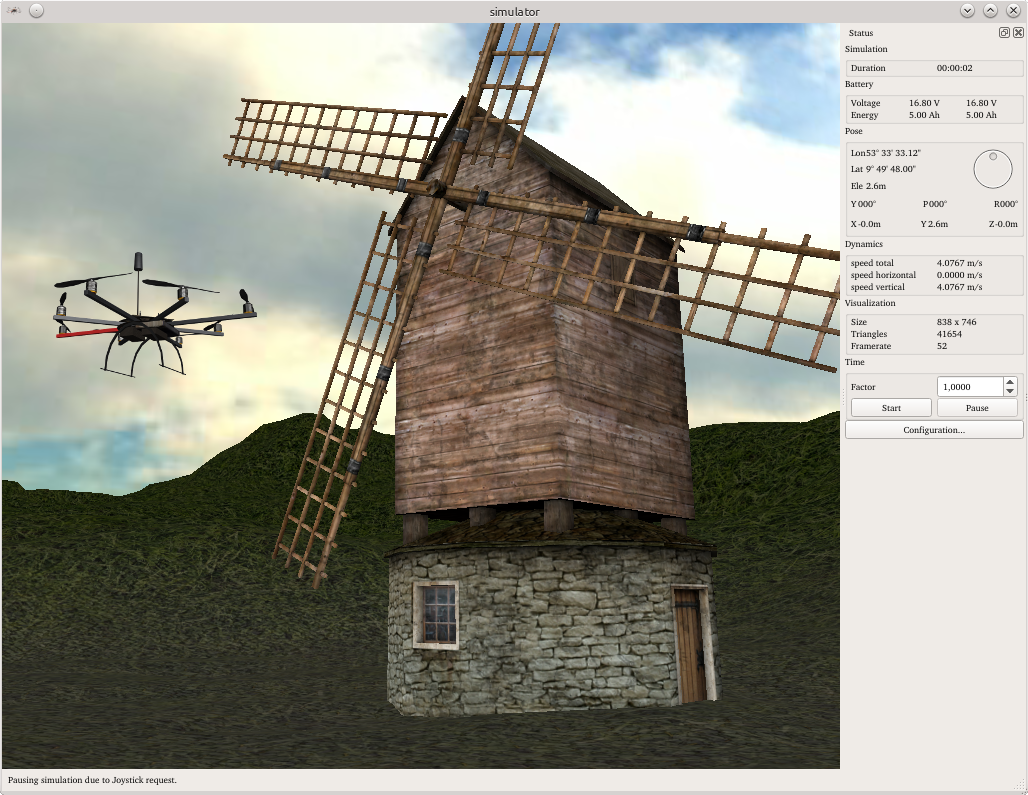
\includegraphics[width=1.0\textwidth]{simulator}
  \caption{Screenshot of the simulator. The UAV can be controlled manually via joystick as well as autonomously using a custom high-level flight-controller that approaches generated waypoints.}
  \label{figure_simulator}
\end{figure}


\newpage\thispagestyle{empty}
% ----------------------------------------------------------------------